\documentclass[11pt,a4paper]{article}

\usepackage[utf8]{inputenc}
\usepackage[T1]{fontenc}
\usepackage[brazil]{babel}
\usepackage{geometry}
\geometry{a4paper, top=20mm, bottom=18mm, left=22mm, right=18mm}

\usepackage{graphicx}
\graphicspath{{../results/figures/}{figures/}}
\usepackage{booktabs}
\usepackage{array}
\usepackage{amsmath}
\usepackage{hyperref}
\usepackage{xcolor}
\usepackage{float}
\usepackage{indentfirst}

\setlength{\parindent}{1.25cm}
\setlength{\parskip}{3pt}

\definecolor{PrimaryBlue}{HTML}{0B3C7D}

\hypersetup{
    colorlinks=true,
    linkcolor=PrimaryBlue,
    urlcolor=PrimaryBlue,
    citecolor=PrimaryBlue
}

\begin{document}

% ==============================================================================
% CABEÇALHO NA 1ª PÁGINA (SEM CAPA SEPARADA - CONFORME SEÇÃO 6 DA PROPOSTA)
% ==============================================================================
\begin{center}
    {\footnotesize\bfseries\color{PrimaryBlue} UNIVERSIDADE DE FORTALEZA (UNIFOR) --- EDUCAÇÃO A DISTÂNCIA (EAD) | REDES NEURAIS ARTIFICIAIS}\\[6pt]
    {\large\bfseries CLASSIFICAÇÃO DE RESÍDUOS SÓLIDOS POR IMAGENS COM REDES NEURAIS ARTIFICIAIS: COMPARAÇÃO ENTRE MLP, CNN, PESOS DE CLASSE, RESOLUÇÃO E TRANSFERÊNCIA DE APRENDIZAGEM COM YOLO}\\[8pt]
    {\small
    \textbf{Equipe:} Caio Cesar da Silva Barros (Matrícula: [XXXXXXX]); Danillo Castro de Sousa (Matrícula: 2523562);\\
    Francisco Vitor Rodrigues Xavier (Matrícula: 2523561); Ian Fonseca Araujo (Matrícula: [XXXXXXX]);\\
    Jose Wesllem Gomes do Nascimento (Matrícula: [XXXXXXX]); Letícia Monteiro Vidal (Matrícula: 2523577)\\[4pt]
    \textbf{Repositório GitHub:} \url{https://github.com/ChicoXavier/trashnet-rna-unifor}
    }
\end{center}
\hrule
\vspace{6pt}

\noindent\textbf{RESUMO:} A triagem automatizada de resíduos sólidos recicláveis é um desafio prático de visão computacional devido à variabilidade visual dos materiais e ao desequilíbrio entre categorias. Este trabalho apresenta um estudo experimental controlado com o conjunto de dados \textit{TrashNet}, após a remoção de 6 amostras pertencentes a 3 pares duplicados via MD5 com rótulos conflitantes, resultando em 2.521 imagens limpas em seis classes (\textit{glass}, \textit{paper}, \textit{cardboard}, \textit{plastic}, \textit{metal} e \textit{trash}), com divisão estratificada fixa (70\% treino, 15\% validação e 15\% teste; semente 42). Foram executados seis experimentos obrigatórios comparando \textit{Multilayer Perceptron} (MLP) e Rede Neural Convolucional (CNN) com e sem pesos de classe em $128 \times 96$ pixels, além da avaliação do efeito da resolução na CNN ($128 \times 96$, $256 \times 192$ e $512 \times 384$) mantendo 28.358 parâmetros via \textit{Global Average Pooling}, sob protocolo uniforme (até 60 épocas, parada antecipada com paciência 10 e mesma aumentação de dados geométrica). Como extensão opcional, aplicou-se transferência de aprendizagem com \textit{YOLO11n-cls} ($224 \times 224$). Nos experimentos obrigatórios, a CNN em $128 \times 96$ com pesos obteve o maior F1 macro de validação (0,7277), atingindo 73,09\% de acurácia e 0,7036 de F1 macro no teste, além de elevar o \textit{recall} da classe minoritária \textit{trash} de 0,45 para 0,60; já a CNN sem pesos em $128 \times 96$ e $256 \times 192$ alcançou 74,67\% de acurácia no teste (F1 macro de 0,7154 e 0,7213), superando amplamente a MLP (34,83\% e 0,2275, com 9,47 milhões de parâmetros). O aumento de resolução para $512 \times 384$ elevou o custo temporal por época em cerca de 22,8 vezes sem melhoria de desempenho (70,98\%). Por fim, o \textit{YOLO11n-cls} atingiu 91,03\% de acurácia e 0,8865 de F1 macro no mesmo conjunto de teste, indicando o impacto do pré-treinamento em larga escala.

\noindent\textbf{Palavras-chave:} Redes Neurais Artificiais. Visão Computacional. TrashNet. Classificação de Resíduos. Transferência de Aprendizagem.

% ==============================================================================
\section{Introdução}
% ==============================================================================

O gerenciamento eficiente de resíduos sólidos urbanos depende diretamente da correta segregação dos materiais recicláveis. No entanto, a triagem manual está sujeita a erros humanos, fadiga e riscos ocupacionais. Nesse contexto, técnicas de aprendizado profundo (\textit{Deep Learning}) e Redes Neurais Artificiais (RNAs) aplicadas à visão computacional e ao reconhecimento de padrões oferecem uma alternativa promissora para identificar automaticamente materiais como vidro, papel, papelão, plástico e metal a partir de imagens digitais (BISHOP; NASRABADI, 2006; GOODFELLOW et al., 2016).

Conforme os fundamentos estudados na disciplina (BARBOSA, 2025), arquiteturas do tipo \textit{Multilayer Perceptron} (MLP) empregam camadas totalmente conectadas e fluxo \textit{feedforward} com funções de ativação suaves e diferenciáveis para aprender mapeamentos não lineares por meio do algoritmo de retropropagação do erro (\textit{backpropagation}), superando as limitações de separabilidade linear do Perceptron Simples e do ADALINE (RUMELHART; HINTON; WILLIAMS, 1986; HAYKIN, 2001; SILVA; SPATTI; FLAUZINO, 2010). Contudo, ao vetorizar imagens RGB diretamente na entrada, a MLP perde a relação geométrica de vizinhança espacial e sofre crescimento excessivo de parâmetros na primeira camada. Em contrapartida, no paradigma de \textit{Deep Learning}, as Redes Neurais Convolucionais (CNNs) preservam a entrada matricial e realizam extração e seleção de características na 1\textsuperscript{a} região por filtros compartilhados e subamostragem (\textit{pooling}), aprendendo mapas hierárquicos de bordas, cantos e contornos antes da etapa de decisão (ZEILER; FERGUS, 2014; GOODFELLOW et al., 2016; BARBOSA, 2025).

O objetivo deste estudo é investigar empiricamente o desempenho, o custo de treinamento e o tempo de inferência de modelos MLP e CNN na classificação das seis classes do conjunto de dados \textit{TrashNet} (YANG; THUNG, 2016). Especificamente, avaliam-se: (i) a diferença arquitetural entre MLP e CNN em $128 \times 96$ pixels; (ii) o efeito da ponderação de classes na função de perda sobre a classe minoritária \textit{trash}; (iii) o custo-benefício do aumento de resolução espacial ($128 \times 96$, $256 \times 192$ e $512 \times 384$) na CNN; e (iv) como objetivo extra opcional, os ganhos obtidos por transferência de aprendizagem com a arquitetura \textit{YOLO11n-cls}.

% ==============================================================================
\section{Materiais e Métodos}
% ==============================================================================

\subsection{Conjunto de Dados e Análise Exploratória}

Utilizou-se como base o arquivo oficial \texttt{dataset-resized.zip} do \textit{TrashNet}, composto originalmente por 2.527 imagens coloridas no formato RGB com dimensão padrão de $512 \times 384$ pixels (largura $\times$ altura). A inspeção automatizada de integridade confirmou zero arquivos corrompidos e 100\% das amostras no modo RGB. Entretanto, a verificação por assinatura criptográfica (MD5) revelou três pares de arquivos idênticos rotulados em categorias distintas: \texttt{plastic152.jpg}/\texttt{glass176.jpg}, \texttt{plastic332.jpg}/\texttt{glass389.jpg} e \texttt{metal91.jpg}/\texttt{glass115.jpg}. Para evitar contaminação e ruído de avaliação entre subconjuntos, todos os 6 arquivos pertencentes a esses pares conflitantes foram removidos \textbf{antes} da divisão dos dados, resultando em um conjunto limpo de \textbf{2.521 imagens} distribuídas em seis classes: \textit{glass} (498), \textit{paper} (594), \textit{cardboard} (403), \textit{plastic} (480), \textit{metal} (409) e \textit{trash} (137).

Visualmente, as fotografias do \textit{TrashNet} foram capturadas em ambiente controlado sobre fundo claro uniforme, com iluminação variável e objetos individuais frequentemente amassados, translúcidos (vidro e plástico) ou com reflexos metálicos (metal e vidro), o que dificulta a discriminação apenas por cor global. A Figura~\ref{fig:dist} exibe a distribuição estratificada após a limpeza e a Figura~\ref{fig:exemplos} apresenta exemplos representativos das seis classes.

\begin{figure}[H]
    \centering
    \caption{Distribuição estratificada das seis classes do TrashNet limpo (2.521 imagens; 70\% treino, 15\% validação, 15\% teste).}
    \label{fig:dist}
    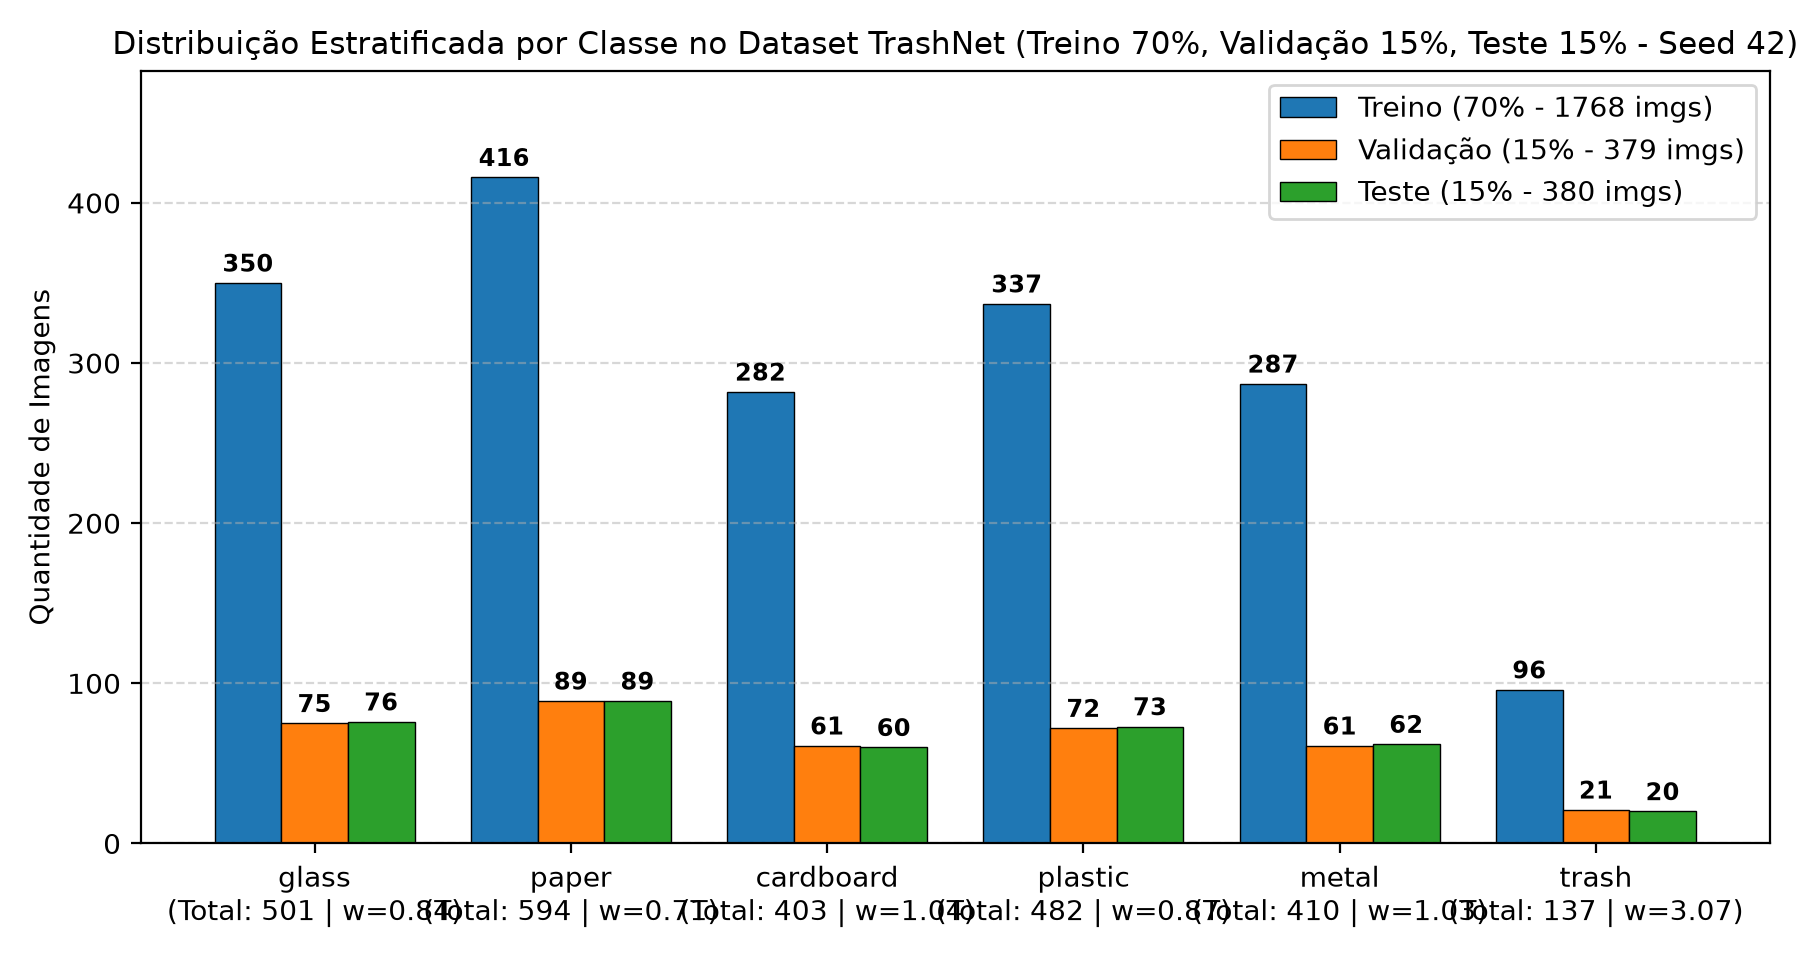
\includegraphics[width=0.88\linewidth]{fig1_distribuicao_classes.png}\\
    {\footnotesize Fonte: Elaborada pelos autores (2026).}
\end{figure}

\begin{figure}[H]
    \centering
    \caption{Exemplos representativos das seis classes no conjunto de treinamento.}
    \label{fig:exemplos}
    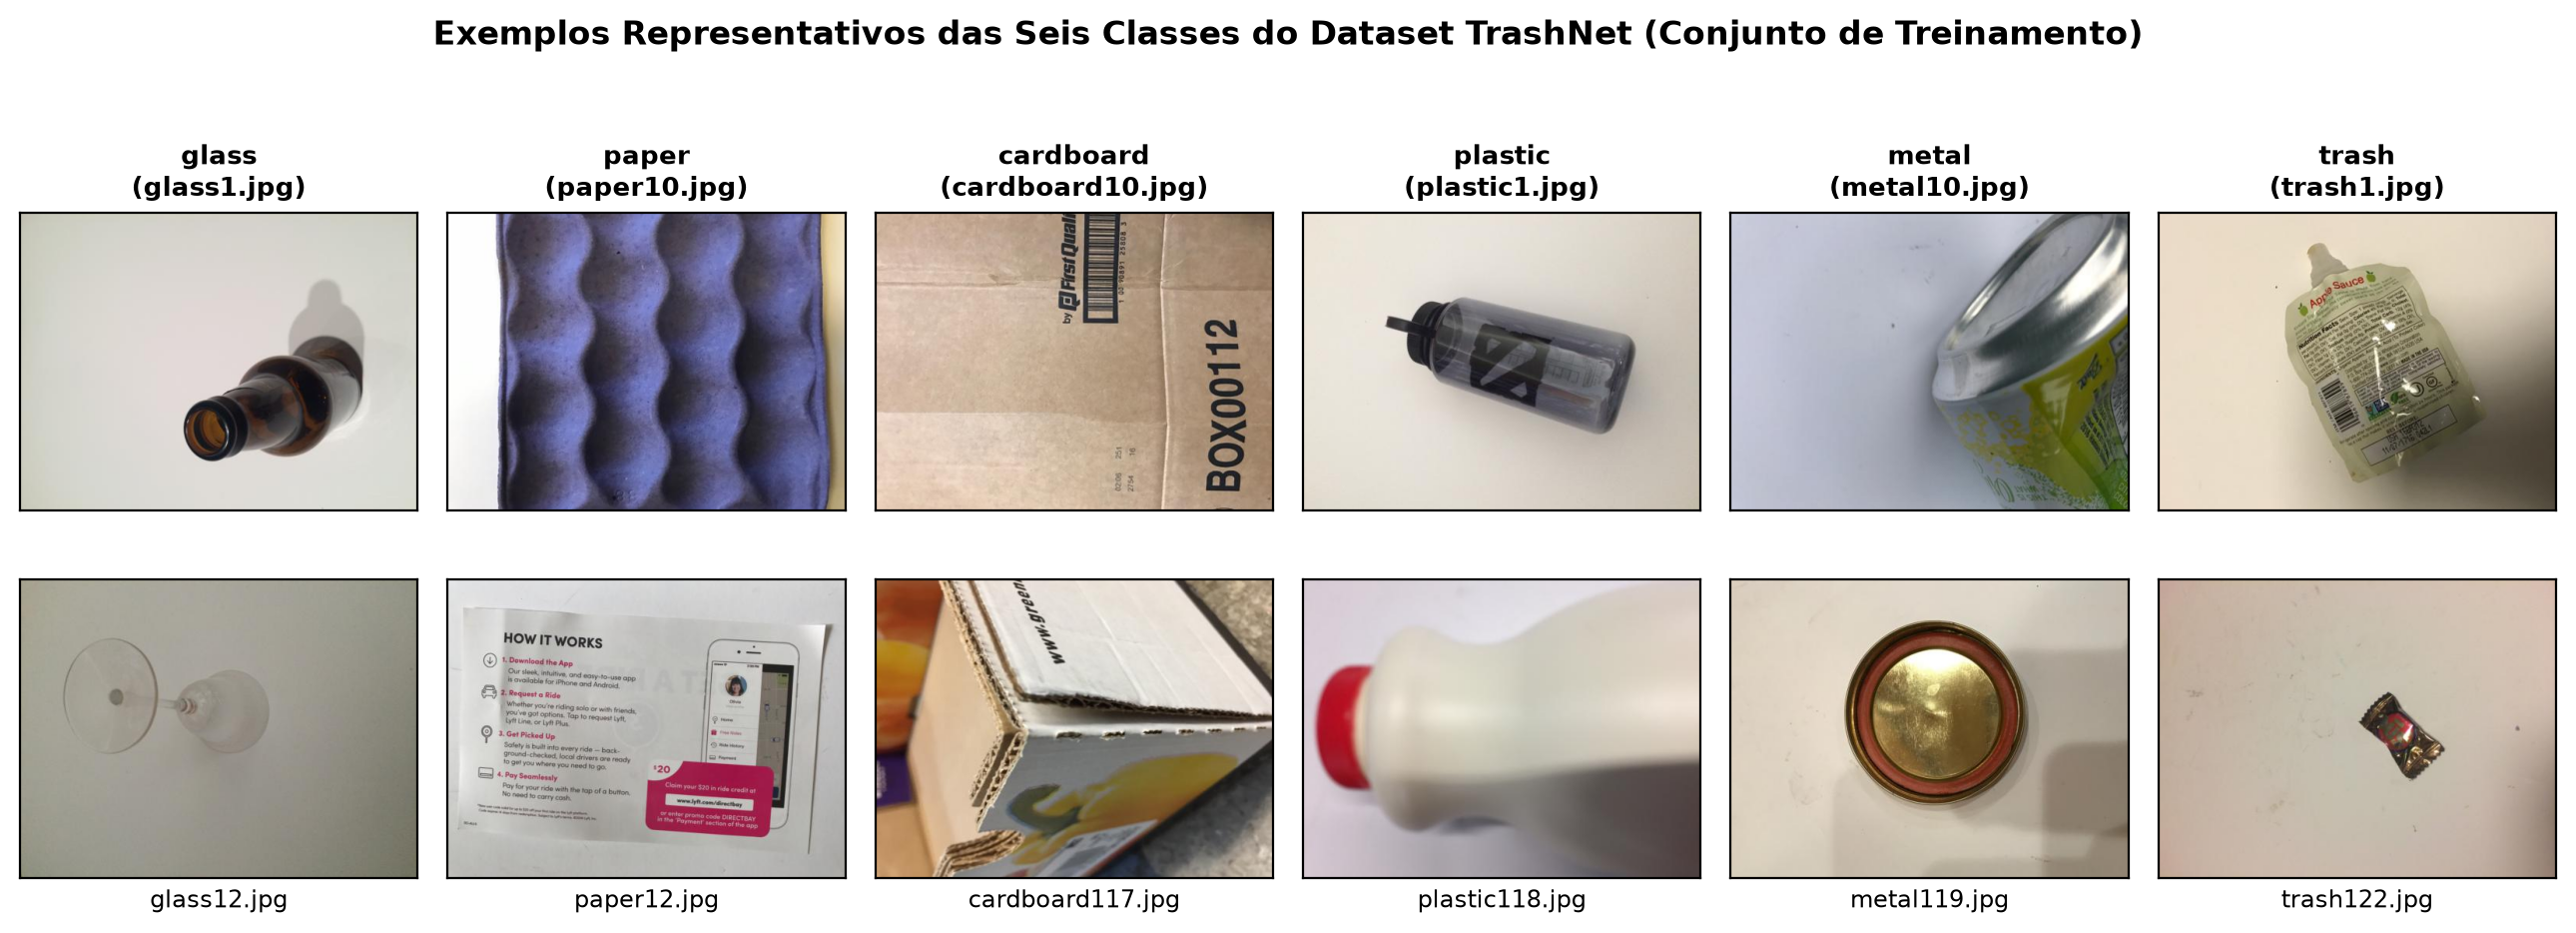
\includegraphics[width=0.95\linewidth]{fig2_exemplos_classes.png}\\
    {\footnotesize Fonte: Elaborada pelos autores a partir de Yang e Thung (2016).}
\end{figure}

\subsection{Divisão Estratificada, Pré-processamento e Prevenção de Vazamento}

Para garantir reprodutibilidade e impedir vazamento de dados (\textit{data leakage}), aplicou-se divisão estratificada fixa com semente \texttt{42} sobre as 2.521 imagens limpas: 1.764 imagens (70\%) para treinamento, 378 (15\%) para validação e 379 (15\%) para teste, mantendo em todos os subconjuntos a proporção original de ${\sim}5{,}43\%$ da classe \textit{trash} (96, 21 e 20 imagens, respectivamente). As imagens foram convertidas para RGB, redimensionadas por interpolação bilinear a partir da referência $512 \times 384$ para $128 \times 96$ e $256 \times 192$ (Figura~\ref{fig:res}) e normalizadas para o intervalo $[0, 1]$ mediante divisão por 255. Para referência estatística exclusiva do treinamento, registraram-se médias RGB de $[0{,}6727;\; 0{,}6397;\; 0{,}6047]$ e desvios padrão de $[0{,}1837;\; 0{,}1828;\; 0{,}1934]$. Para manter comparação justa entre arquiteturas, aplicou-se exatamente a mesma aumentação de dados geométrica leve (espelhamento horizontal com $p = 0{,}5$ e rotação aleatória de $\pm 10^\circ$ com $p = 0{,}5$) tanto para a MLP quanto para as CNNs, exclusivamente durante o treinamento.

\begin{figure}[H]
    \centering
    \caption{Comparação visual da amostra \texttt{metal107.jpg} nas três resoluções experimentais ($\text{L} \times \text{A}$).}
    \label{fig:res}
    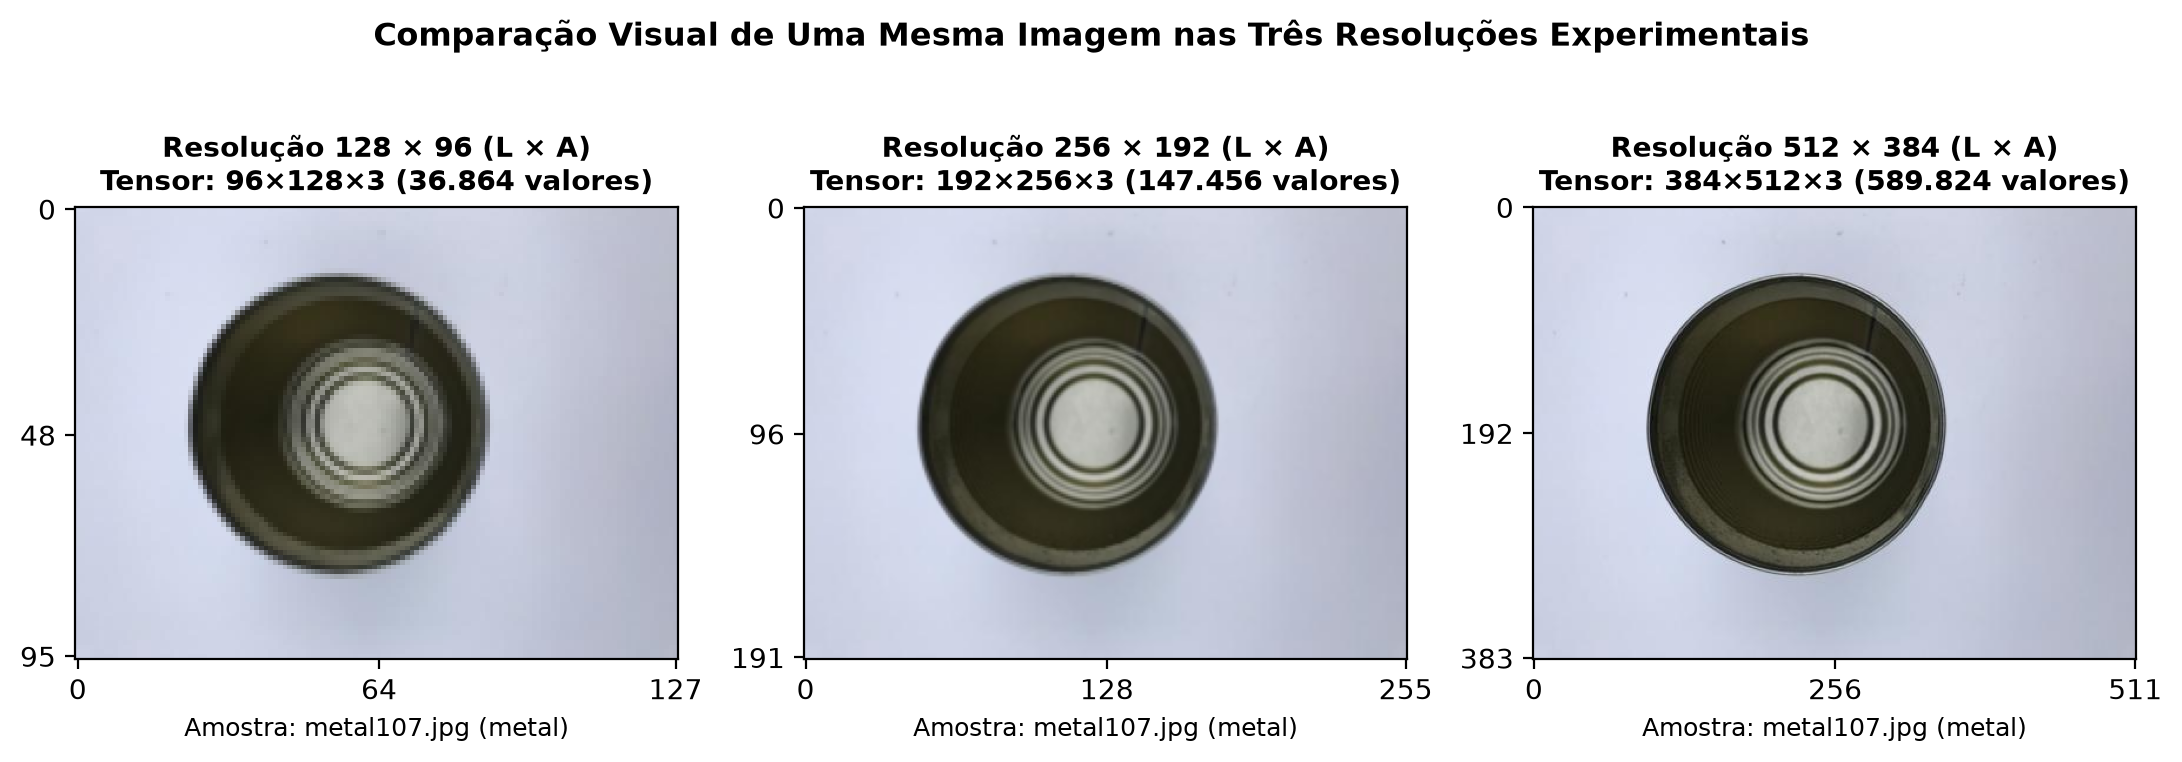
\includegraphics[width=0.92\linewidth]{fig3_comparacao_resolucoes.png}\\
    {\footnotesize Fonte: Elaborada pelos autores (2026).}
\end{figure}

\subsection{Arquitetura, Topologia e Protocolo dos Experimentos Controlados}

Distinguindo \textit{arquitetura} (fluxo macroscópico do sinal) de \textit{topologia} (hiperparâmetros internos definidos pelo projetista), todos os modelos obrigatórios foram implementados em PyTorch (PASZKE et al., 2019) e treinados do zero em modo \textit{offline} por mini-lotes (\textit{batch size} = 32) com semente fixa (\texttt{42}), limite uniforme de \textbf{60 épocas}, otimizador \textbf{Adam} (taxa de aprendizagem inicial $lr = 10^{-3}$, decaimento de pesos $10^{-4}$, escalonador \textit{ReduceLROnPlateau} com fator 0,5 e paciência 3), função de perda Entropia Cruzada (\textit{CrossEntropyLoss}) e ativação \textbf{ReLU} ($g(u) = \max(0, u)$) nas camadas intermediárias --- escolhida para evitar operações exponenciais e reduzir a saturação das sigmoidais. Adotou-se \textbf{Parada Antecipada (\textit{Early Stopping})} uniforme com \textbf{paciência de 10 épocas} nos seis experimentos obrigatórios, monitorando o \textbf{F1 macro de validação} e restaurando os pesos da melhor época antes da avaliação única no conjunto de teste (BARBOSA, 2025).

\begin{itemize}
    \item \textbf{MLP ($128 \times 96$):} Vetorização da imagem RGB ($96 \times 128 \times 3 = 36.864$ entradas), duas camadas ocultas densas (256 e 128 neurônios) com ReLU, \textit{Dropout} (taxa 0,20, desativando 20\% dos neurônios no treino para distribuir o conhecimento) e camada de saída com 6 neurônios (9.471.110 parâmetros).
    \item \textbf{CNN ($128 \times 96$, $256 \times 192$ e $512 \times 384$):} Estruturada em duas regiões funcionais: (1) \textit{Extração e Seleção de Características} --- três blocos sequenciais de Convolução 2D (16, 32 e 64 filtros $3\times 3$ com \textit{padding} 1 e \textit{stride} 2 no primeiro bloco), \textit{BatchNorm2d}, ReLU e \textit{MaxPooling2D} ($2\times 2$), culminando em \textit{Global Average Pooling} (\texttt{AdaptiveAvgPool2d(1)}); e (2) \textit{Decisão} --- vetorização (\texttt{Flatten}) seguida de MLP densa (64 neurônios ReLU + \textit{Dropout} 0,20 + 6 saídas), mantendo exatamente \textbf{28.358 parâmetros} nas três resoluções.
    \item \textbf{Pesos de Classe:} Nos Experimentos 2 (MLP) e 4 (CNN), utilizaram-se pesos inversamente proporcionais à frequência calculados apenas no treino: $w_c = N_{\text{treino}} / (6 \cdot N_{\text{treino},c})$ (BISHOP; NASRABADI, 2006), resultando em \textit{glass} = 0,8448; \textit{paper} = 0,7067; \textit{cardboard} = 1,0426; \textit{plastic} = 0,8750; \textit{metal} = 1,0280; e \textit{trash} = 3,0625.
\end{itemize}

\textbf{Objetivo Extra (YOLO11n-cls):} Aplicou-se transferência de aprendizagem com o modelo \texttt{yolo11n-cls.pt} (Ultralytics 8.4.216, pré-treinado no ImageNet-1K, 1.538.790 parâmetros) no modo \textit{classify} (JOCHER; CHAURASIA; QIU, 2024), preservando exatamente os mesmos diretórios de treino, validação e teste da semente 42 sobre as 2.521 imagens limpas. O ajuste fino ocorreu em $224 \times 224$ pixels por 20 épocas com otimizador AdamW ($lr_0 = 0{,}001$, lote 32) e aumentação padrão do \textit{YOLO classify} apenas no treino.

\textbf{Hardware e Medição de Custo:} Os experimentos foram disparados remotamente a partir da estação Linux local e executados em CPU \texttt{Intel(R) Core(TM) i7-4850HQ CPU @ 2.30GHz} (16,0~GB de RAM, sistema operacional \texttt{Darwin 20.6.0} / macOS, Python 3.11.18 e PyTorch 2.2.2), sem GPU CUDA disponível. Registrou-se o pico de memória RAM (RSS) via biblioteca \texttt{psutil}, cronometrou-se exclusivamente o laço de treinamento e validação por época via \texttt{time.perf\_counter()} (excluindo download, leitura de disco e redimensionamento prévio) e mediu-se o tempo médio de inferência por imagem (ms/img) sobre todas as 379 amostras do teste na mesma CPU.

% ==============================================================================
\section{Resultados}
% ==============================================================================

A Tabela~\ref{tab:geral} consolida as métricas de desempenho (validação e teste), o custo de treinamento e a latência média de inferência por imagem dos seis experimentos obrigatórios e do experimento bônus com YOLO11n-cls. A Tabela~\ref{tab:classe} detalha precisão, \textit{recall}, F1 e suporte por classe no conjunto de teste limpo (379 amostras), utilizando \texttt{zero\_division=0} quando uma classe não recebe nenhuma predição.

\begin{table}[H]
\centering
\scriptsize
\caption{Desempenho comparativo, custo e inferência no TrashNet limpo (Seed = 42).}
\label{tab:geral}
\setlength{\tabcolsep}{2.5pt}
\begin{tabular}{lccccccccccc}
\toprule
\textbf{Experimento} & \textbf{Res.} & \textbf{Pesos} & \textbf{Parâm.} & \textbf{Tam.(MB)} & \textbf{Ép.} & \textbf{T.Tot(s)} & \textbf{T/Ép(s)} & \textbf{Inf.(ms)} & \textbf{RAM(MB)} & \textbf{Val F1} & \textbf{Teste Acc / F1} \\
\midrule
Exp 1: MLP & 128$\times$96 & Não & 9.471.110 & 36,13 & 2/12 & 70,97 & 5,91 & 0,24 & 963,0 & 0,2000 & 34,83\% / 0,2275 \\
Exp 2: MLP & 128$\times$96 & Sim & 9.471.110 & 36,13 & 1/11 & 64,91 & 5,90 & 0,23 & 963,7 & 0,0785 & 25,86\% / 0,1100 \\
Exp 3: CNN & 128$\times$96 & Não & 28.358 & 0,12 & 42/52 & 213,74 & 4,11 & 0,62 & 846,0 & 0,7059 & 74,67\% / 0,7154 \\
\textbf{Exp 4: CNN} & \textbf{128$\times$96} & \textbf{Sim} & \textbf{28.358} & \textbf{0,12} & \textbf{39/49} & \textbf{200,80} & \textbf{4,10} & \textbf{0,82} & \textbf{675,1} & \textbf{0,7277} & \textbf{73,09\% / 0,7036} \\
Exp 5: CNN & 256$\times$192 & Não & 28.358 & 0,12 & 45/55 & 1.206,65 & 21,94 & 3,74 & 2.112,3 & 0,6764 & 74,67\% / 0,7213 \\
Exp 6: CNN & 512$\times$384 & Não & 28.358 & 0,12 & 23/33 & 3.088,45 & 93,59 & 18,07 & 6.439,6 & 0,6212 & 70,98\% / 0,6582 \\
\textbf{Exp 7: YOLO11n-cls} & \textbf{224$\times$224} & \textbf{Pré-tr.} & \textbf{1.538.790} & \textbf{3,05} & \textbf{20/20} & \textbf{2.462,58} & \textbf{123,13} & \textbf{16,70} & \textbf{454,4} & \textbf{0,9233*} & \textbf{91,03\% / 0,8865} \\
\bottomrule
\end{tabular}\\
{\footnotesize Fonte: Elaborada pelos autores (2026). *Para o YOLO11n-cls, registra-se a acurácia Top-1 de validação reportada pelo Ultralytics.}
\end{table}

\begin{table}[H]
\centering
\footnotesize
\caption{Métricas por classe no conjunto de teste limpo (379 imagens; \texttt{zero\_division=0}).}
\label{tab:classe}
\setlength{\tabcolsep}{3pt}
\begin{tabular}{lcccccc}
\toprule
\textbf{Experimento} & \textbf{glass (75)} & \textbf{paper (89)} & \textbf{cardboard (61)} & \textbf{plastic (72)} & \textbf{metal (62)} & \textbf{trash (20)} \\
 & P / R / F1 & P / R / F1 & P / R / F1 & P / R / F1 & P / R / F1 & P / R / F1 \\
\midrule
Exp 1: MLP (128$\times$96) & 0,50/0,01/0,03 & 0,28/0,97/0,44 & 0,92/0,38/0,53 & 0,46/0,31/0,37 & 0,00/0,00/0,00 & 0,00/0,00/0,00 \\
Exp 2: MLP (128$\times$96, Pesos) & 0,00/0,00/0,00 & 0,24/1,00/0,39 & 1,00/0,08/0,15 & 0,25/0,01/0,03 & 0,75/0,05/0,09 & 0,00/0,00/0,00 \\
Exp 3: CNN (128$\times$96) & 0,65/0,85/0,74 & 0,76/0,88/0,82 & 0,91/0,85/0,88 & 0,72/0,58/0,65 & 0,76/0,61/0,68 & 0,64/0,45/0,53 \\
\textbf{Exp 4: CNN (128$\times$96, Pesos)} & \textbf{0,66/0,81/0,73} & \textbf{0,80/0,80/0,80} & \textbf{0,93/0,82/0,87} & \textbf{0,69/0,61/0,65} & \textbf{0,78/0,63/0,70} & \textbf{0,40/0,60/0,48} \\
Exp 5: CNN (256$\times$192) & 0,61/0,80/0,69 & 0,80/0,84/0,82 & 0,93/0,89/0,91 & 0,71/0,65/0,68 & 0,74/0,63/0,68 & 0,89/0,40/0,55 \\
Exp 6: CNN (512$\times$384) & 0,60/0,79/0,68 & 0,67/0,91/0,77 & 0,87/0,87/0,87 & 0,70/0,60/0,65 & 0,88/0,45/0,60 & 0,83/0,25/0,38 \\
\textbf{Exp 7: YOLO11n-cls} & \textbf{0,95/0,95/0,95} & \textbf{0,93/0,90/0,91} & \textbf{0,98/0,93/0,96} & \textbf{0,89/0,89/0,89} & \textbf{0,89/0,94/0,91} & \textbf{0,65/0,75/0,70} \\
\bottomrule
\end{tabular}\\
{\footnotesize Fonte: Elaborada pelos autores (2026). Valores abreviados (P = Precisão, R = Recall, F1 = F1-score).}
\end{table}

As curvas de perda e acurácia por época dos seis experimentos obrigatórios são exibidas na Figura~\ref{fig:curvas}, e as matrizes de confusão no conjunto de teste constam na Figura~\ref{fig:cm}.

\begin{figure}[H]
    \centering
    \caption{Curvas de aprendizagem (perda e acurácia de treino e validação) dos seis experimentos obrigatórios.}
    \label{fig:curvas}
    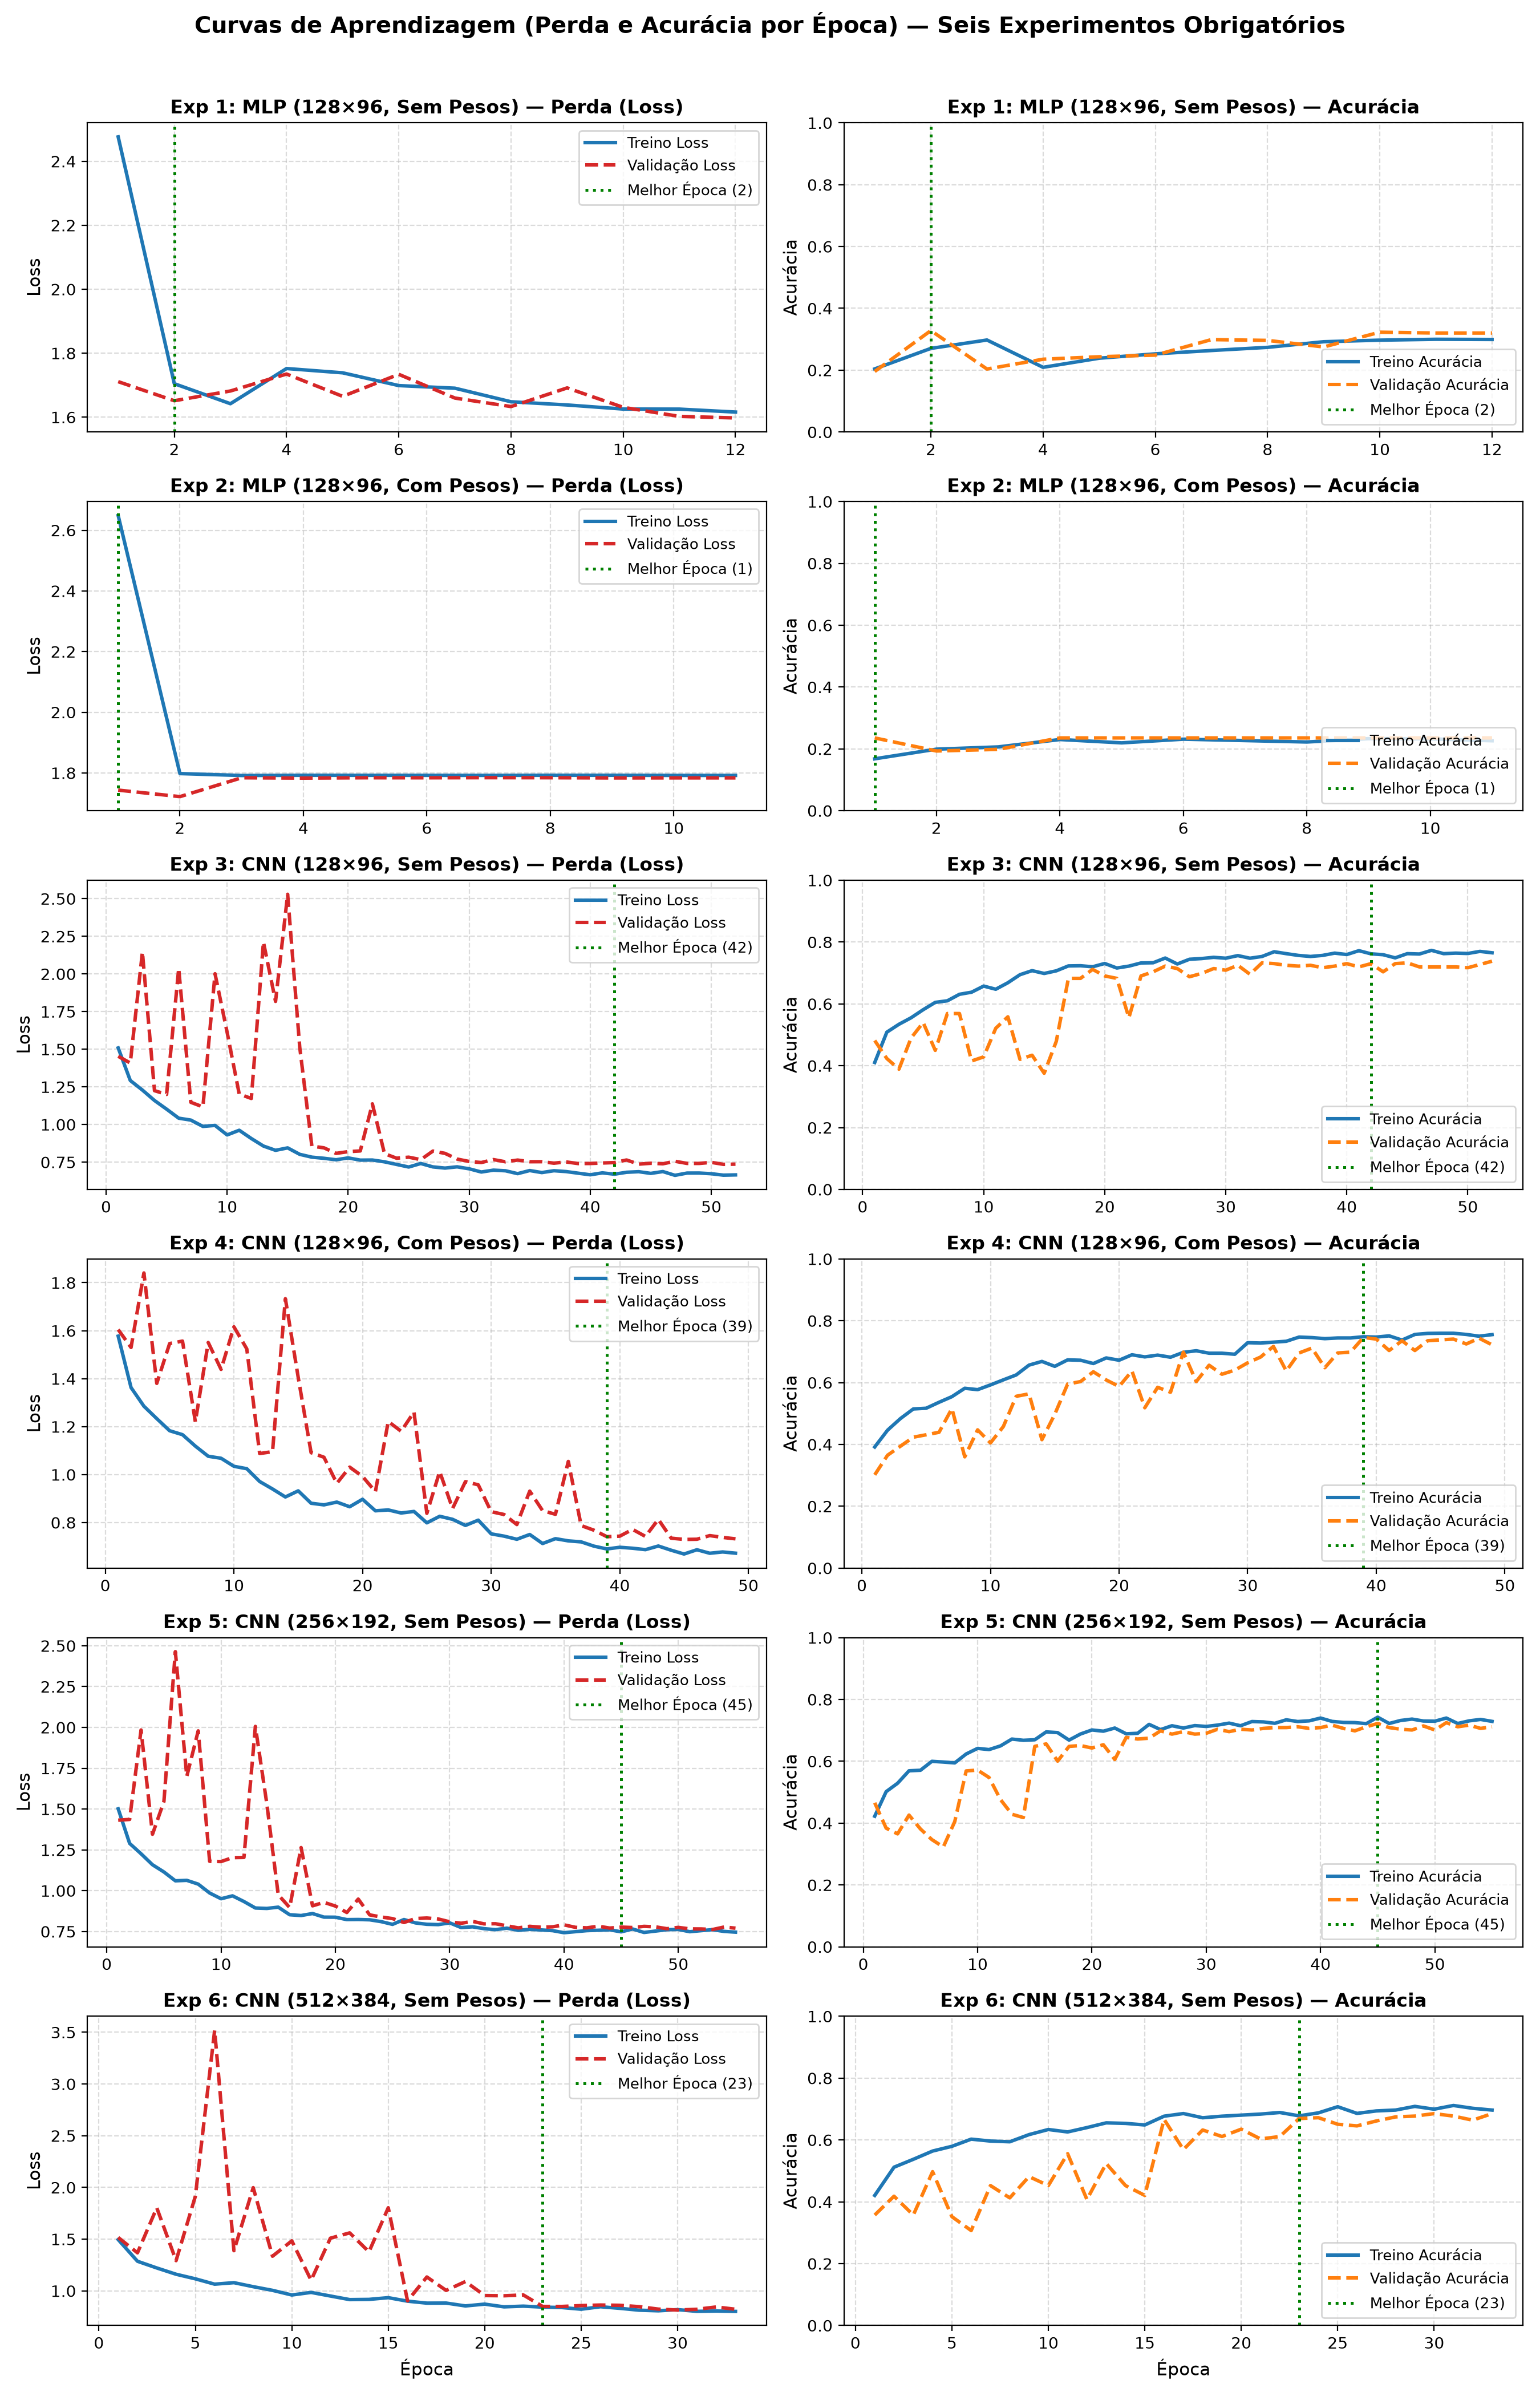
\includegraphics[width=0.98\linewidth, height=0.72\textheight, keepaspectratio]{fig4_curvas_aprendizagem_6exp.png}\\
    {\footnotesize Fonte: Elaborada pelos autores (2026).}
\end{figure}

\begin{figure}[H]
    \centering
    \caption{Matrizes de confusão no conjunto de teste (contagens e porcentagens por linha).}
    \label{fig:cm}
    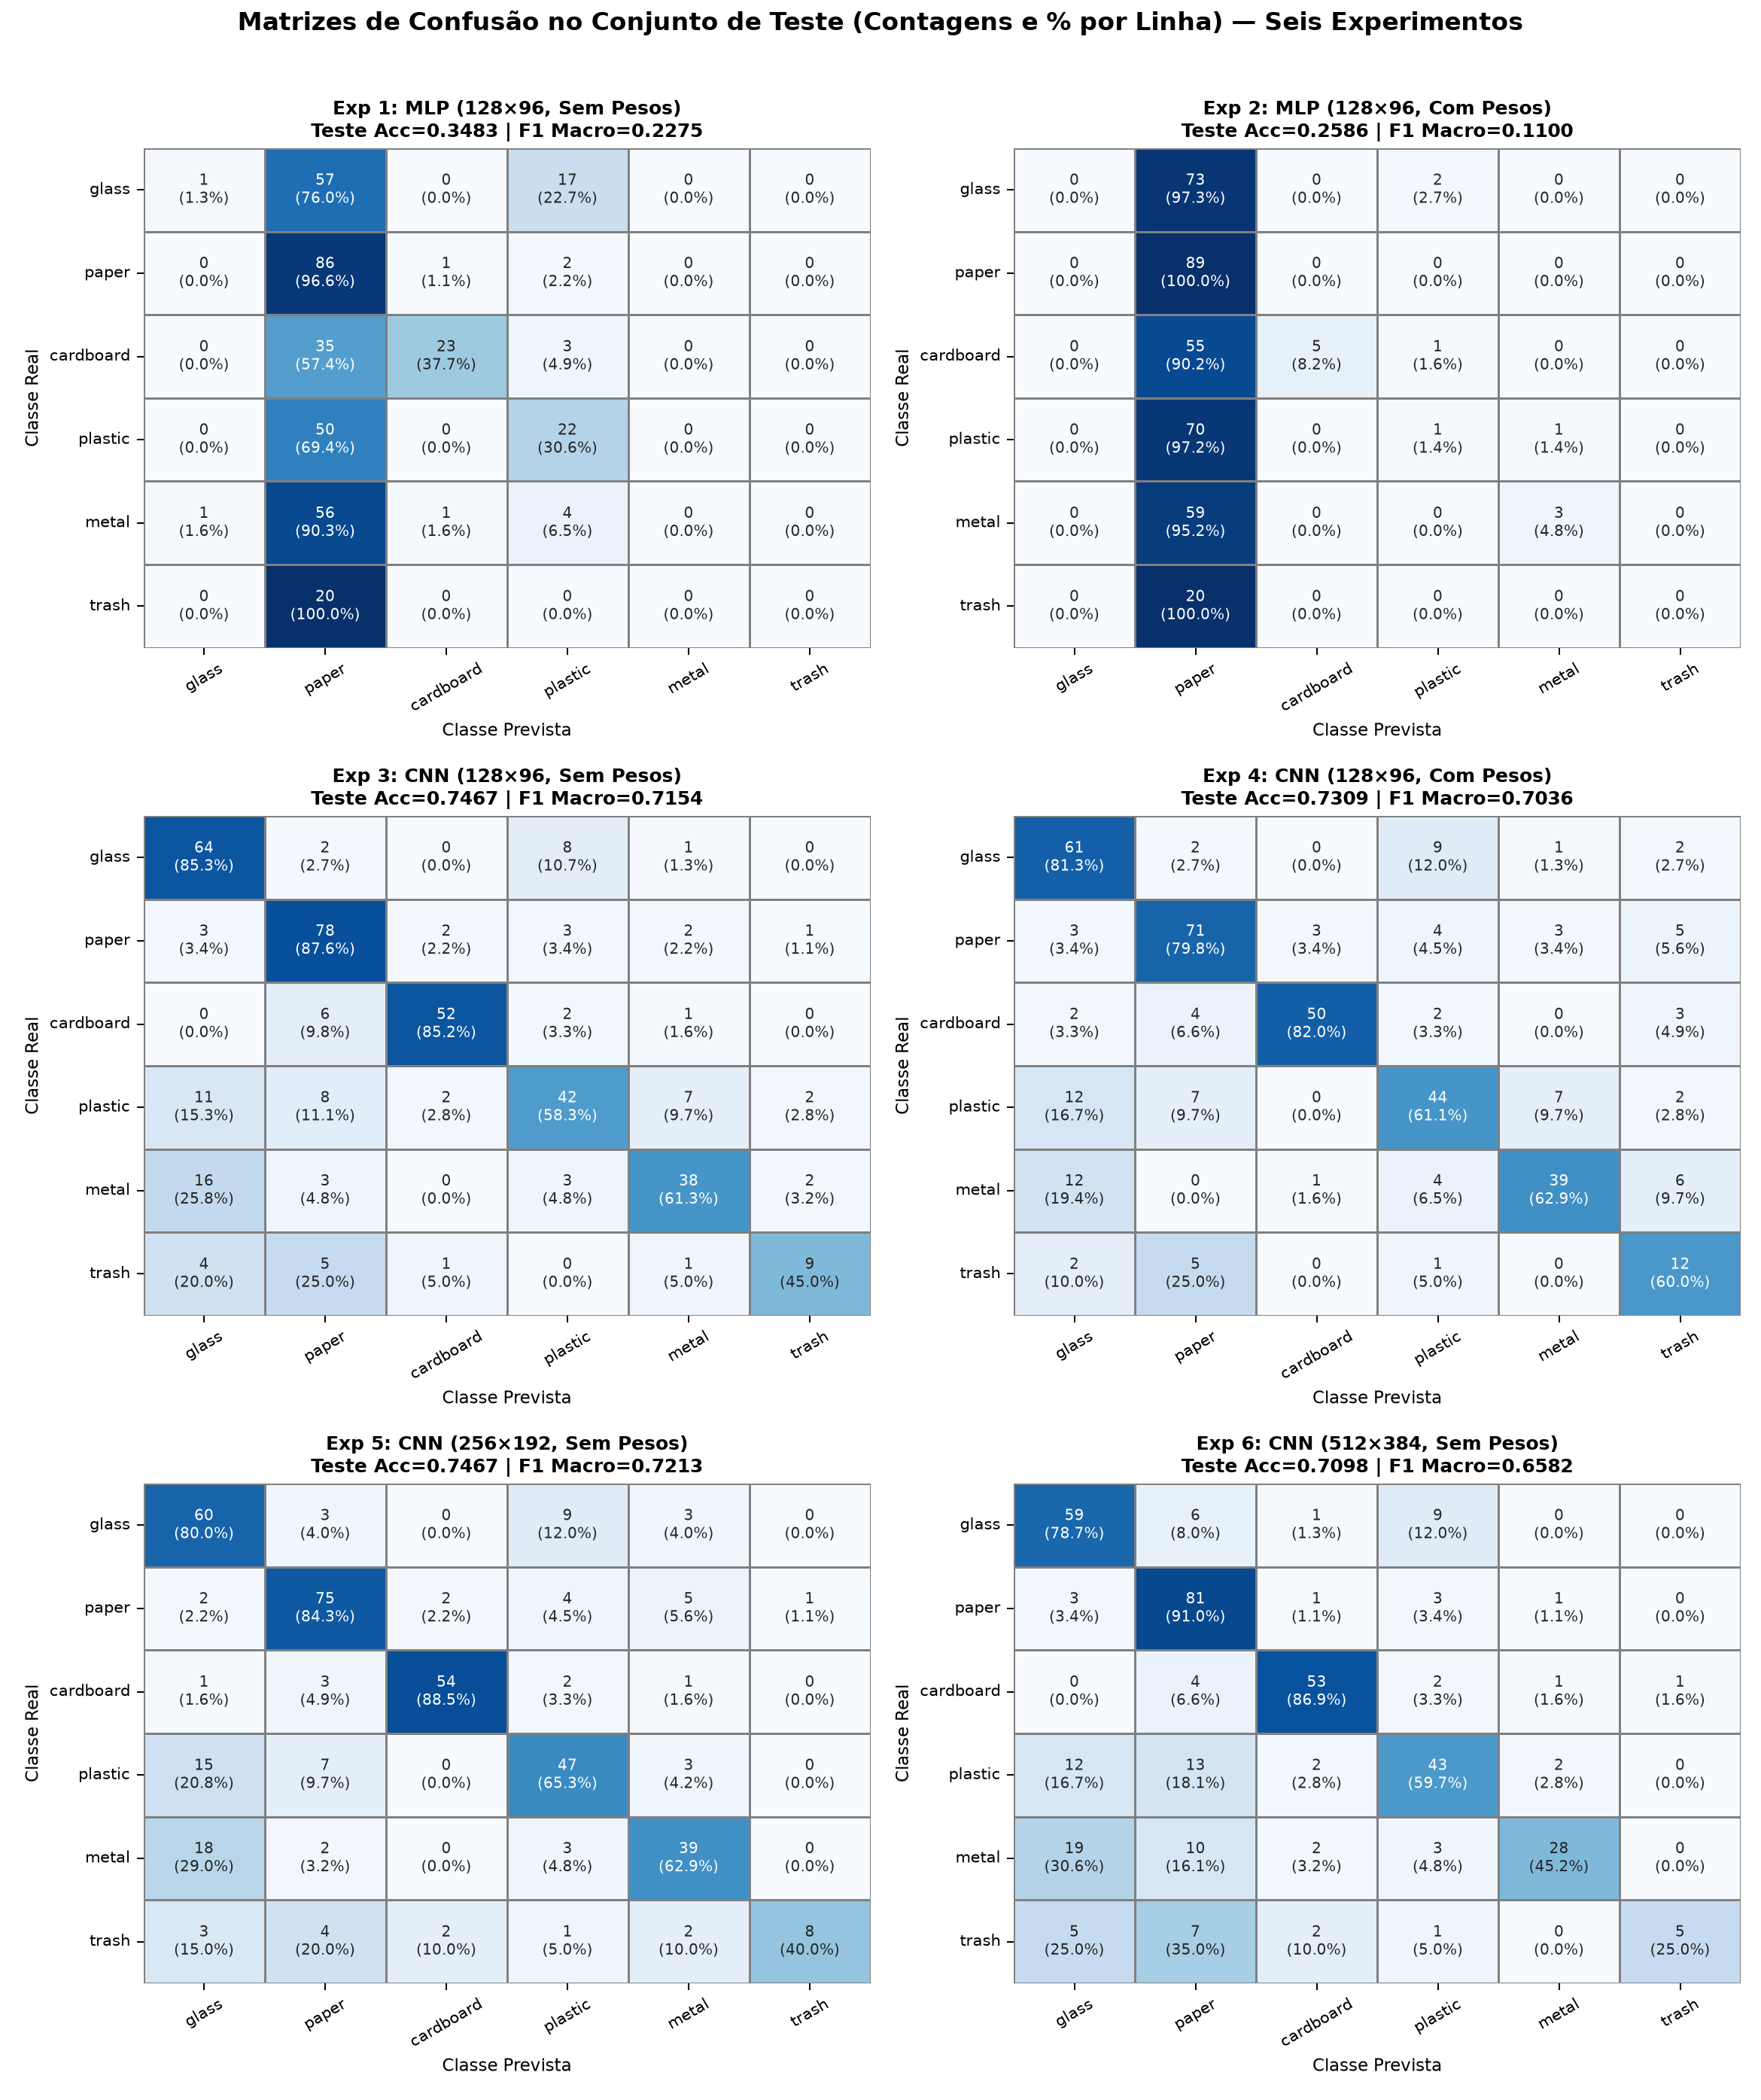
\includegraphics[width=0.98\linewidth, height=0.68\textheight, keepaspectratio]{fig5_matrizes_confusao_6exp.png}\\
    {\footnotesize Fonte: Elaborada pelos autores (2026).}
\end{figure}

A Figura~\ref{fig:res_eff} ilustra o efeito do aumento de resolução na CNN sem pesos de classe (Experimentos 3, 5 e 6), e a Figura~\ref{fig:erros} apresenta a análise dos erros do modelo obrigatório de maior F1 macro na validação (\textbf{Exp 4: CNN $128 \times 96$ com pesos}, Val F1 Macro = 0,7277; 102 erros e 277 acertos em 379 amostras). Por fim, a Figura~\ref{fig:yolo} exibe a avaliação do objetivo extra com \textbf{YOLO11n-cls} (91,03\% de acurácia, 345 acertos e 34 erros no teste).

\begin{figure}[H]
    \centering
    \caption{Efeito da resolução na CNN sem pesos: (a) desempenho no teste e (b) custo temporal.}
    \label{fig:res_eff}
    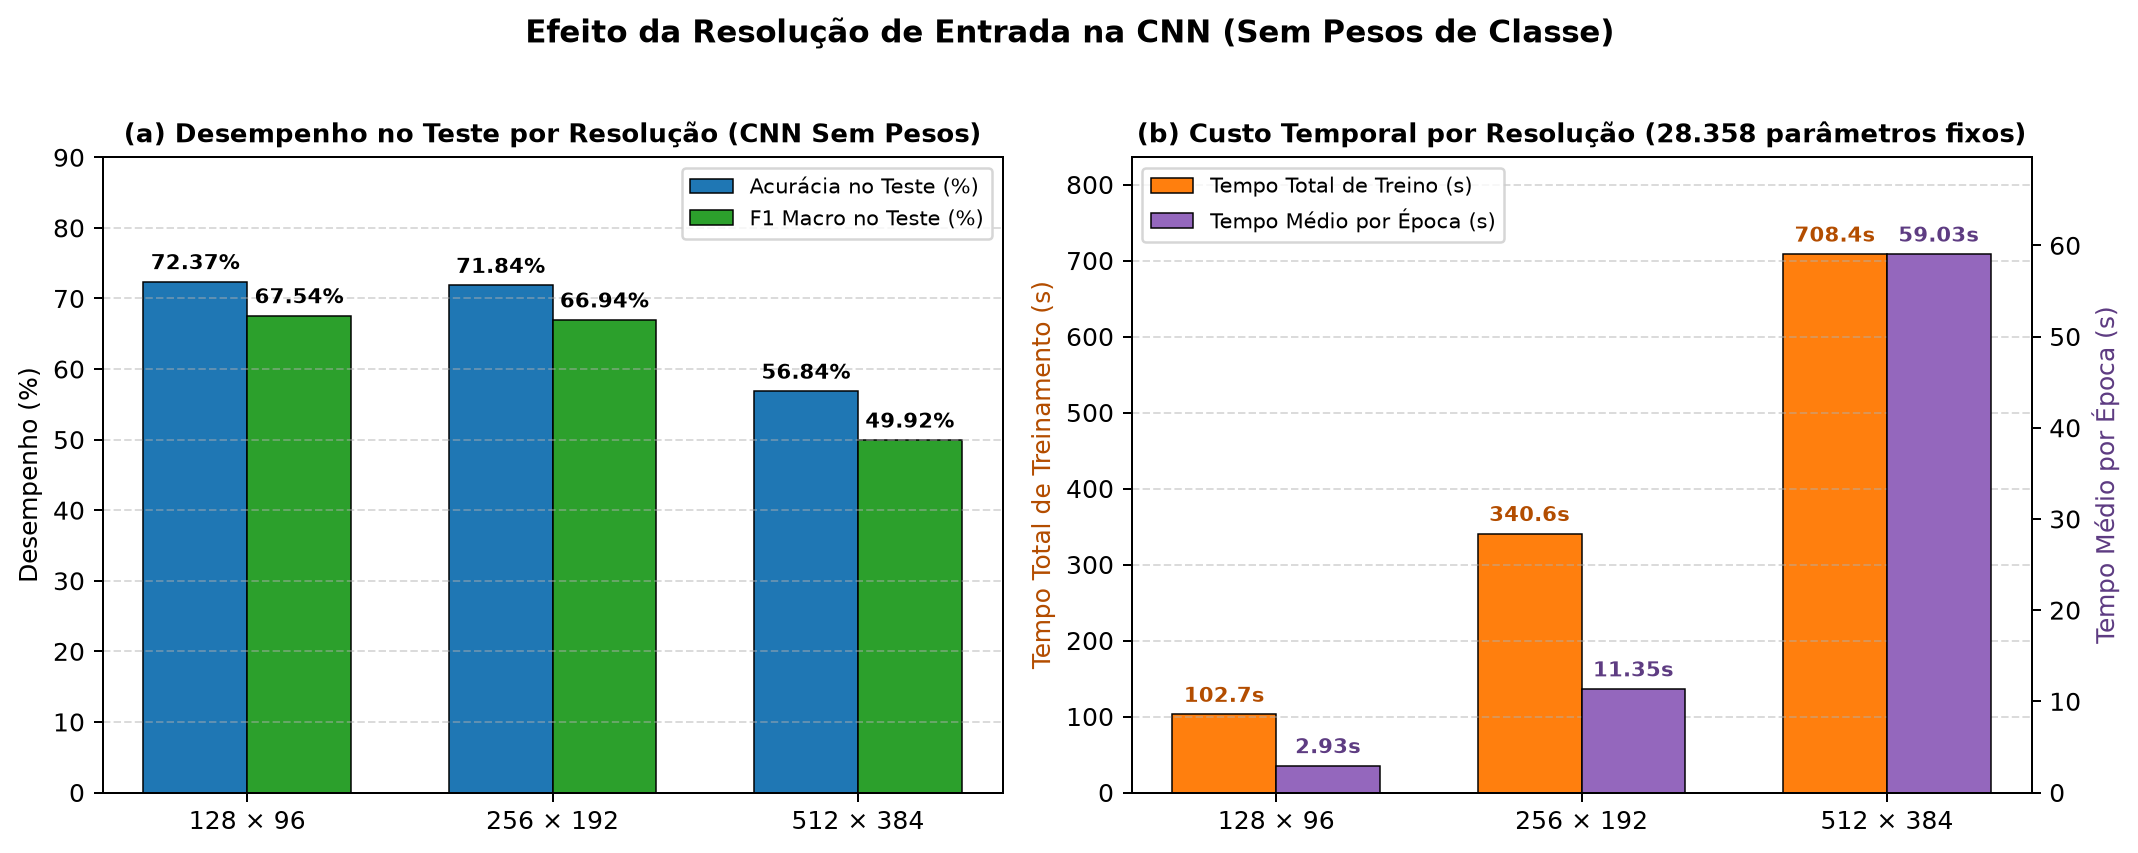
\includegraphics[width=0.95\linewidth]{fig6_efeito_resolucao_cnn.png}\\
    {\footnotesize Fonte: Elaborada pelos autores (2026).}
\end{figure}

\begin{figure}[H]
    \centering
    \caption{Análise de erros do melhor modelo obrigatório na validação (Exp 4: CNN $128 \times 96$ com pesos).}
    \label{fig:erros}
    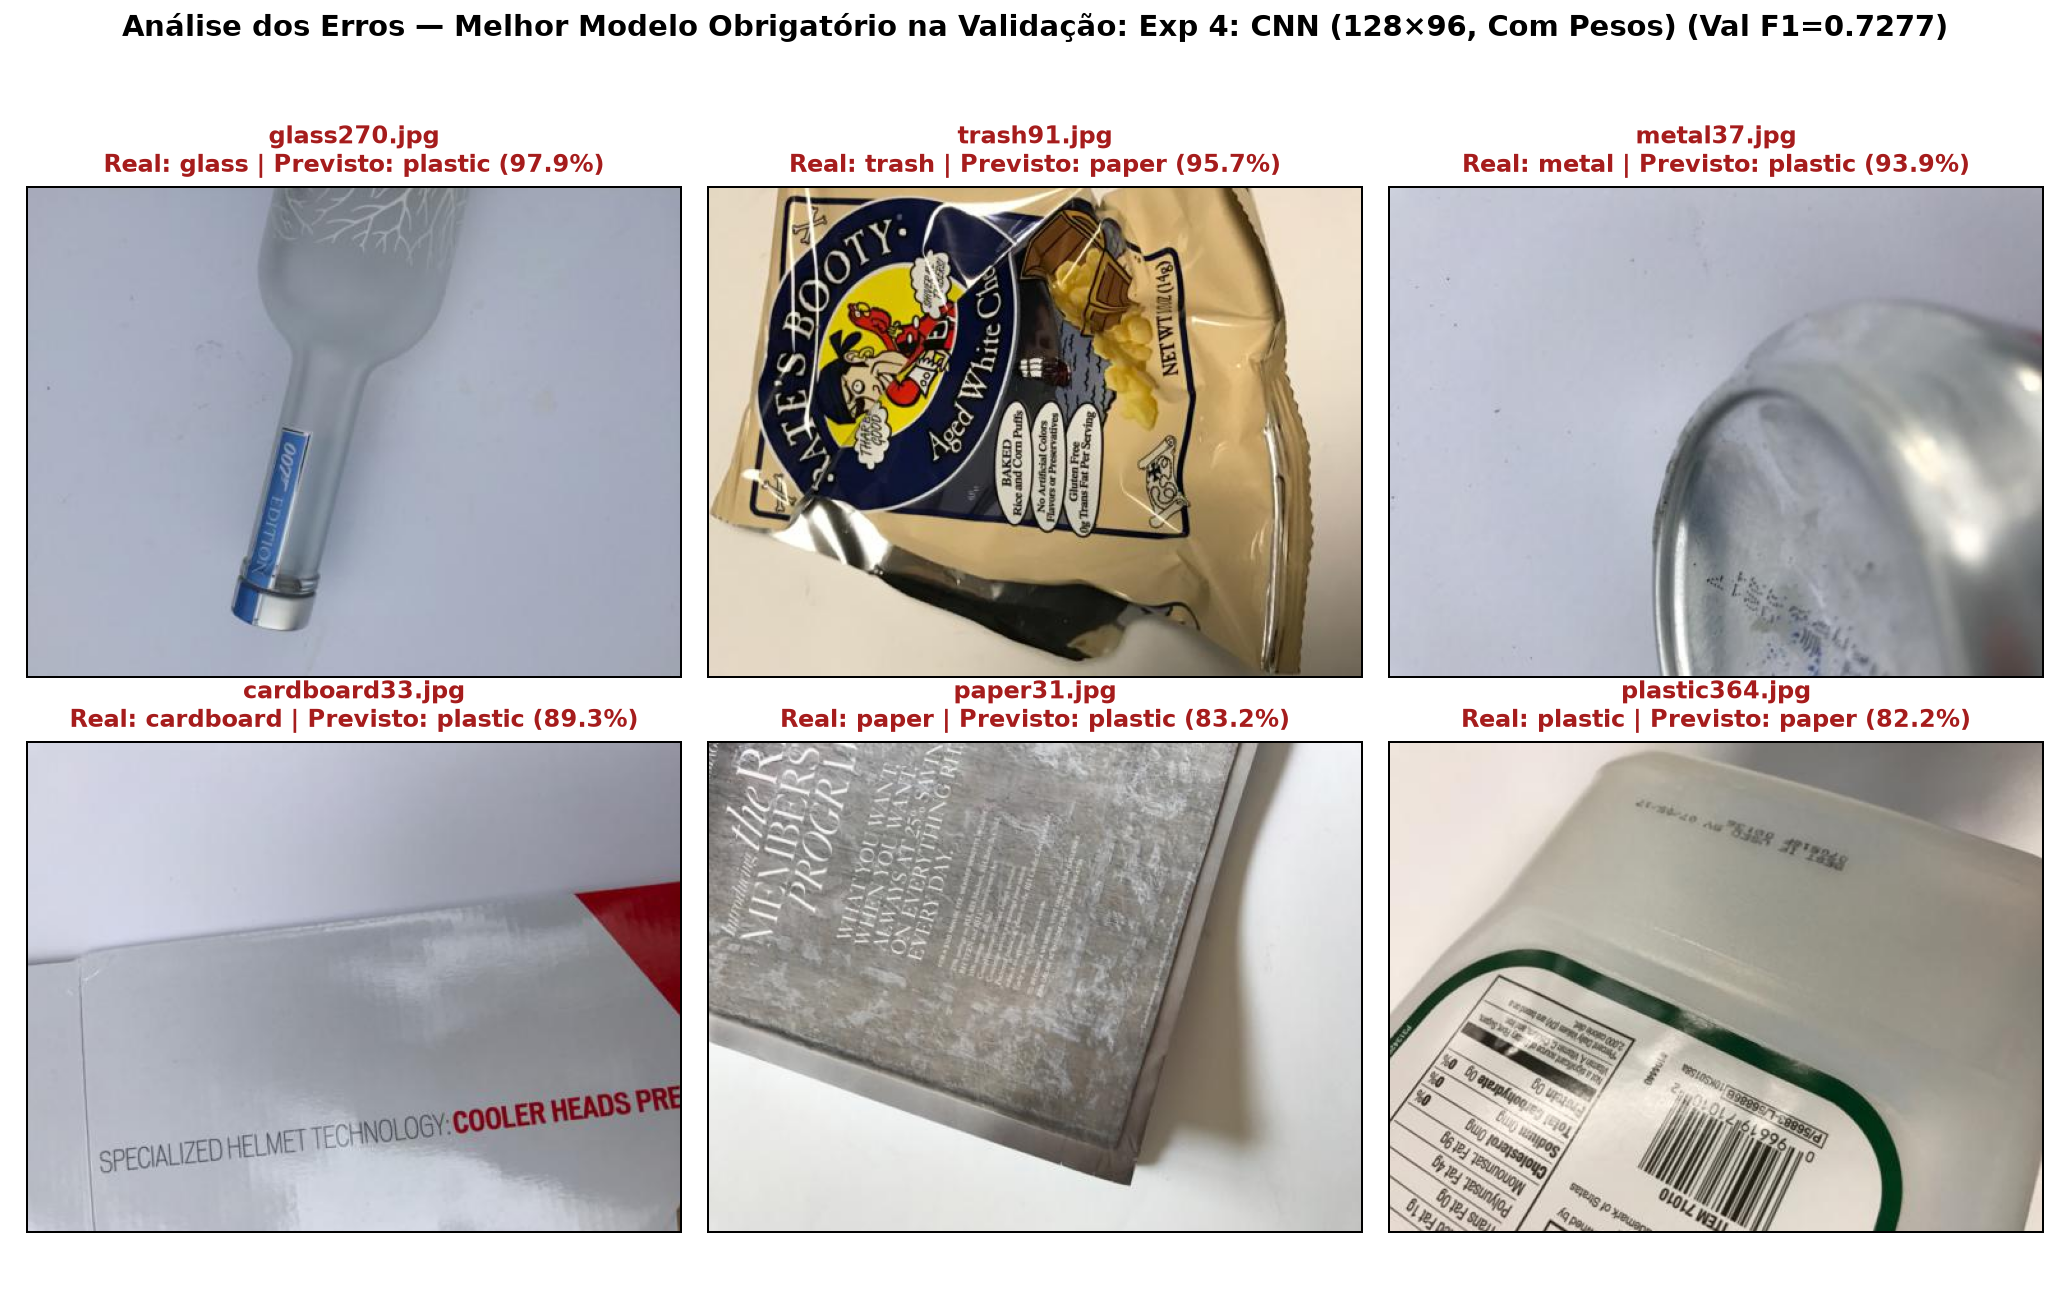
\includegraphics[width=0.90\linewidth]{fig7_analise_erros_melhor_modelo.png}\\
    {\footnotesize Fonte: Elaborada pelos autores (2026).}
\end{figure}

\begin{figure}[H]
    \centering
    \caption{Avaliação do objetivo extra com YOLO11n-cls ($224 \times 224$): perda, acurácia Top-1 e matriz de confusão no teste.}
    \label{fig:yolo}
    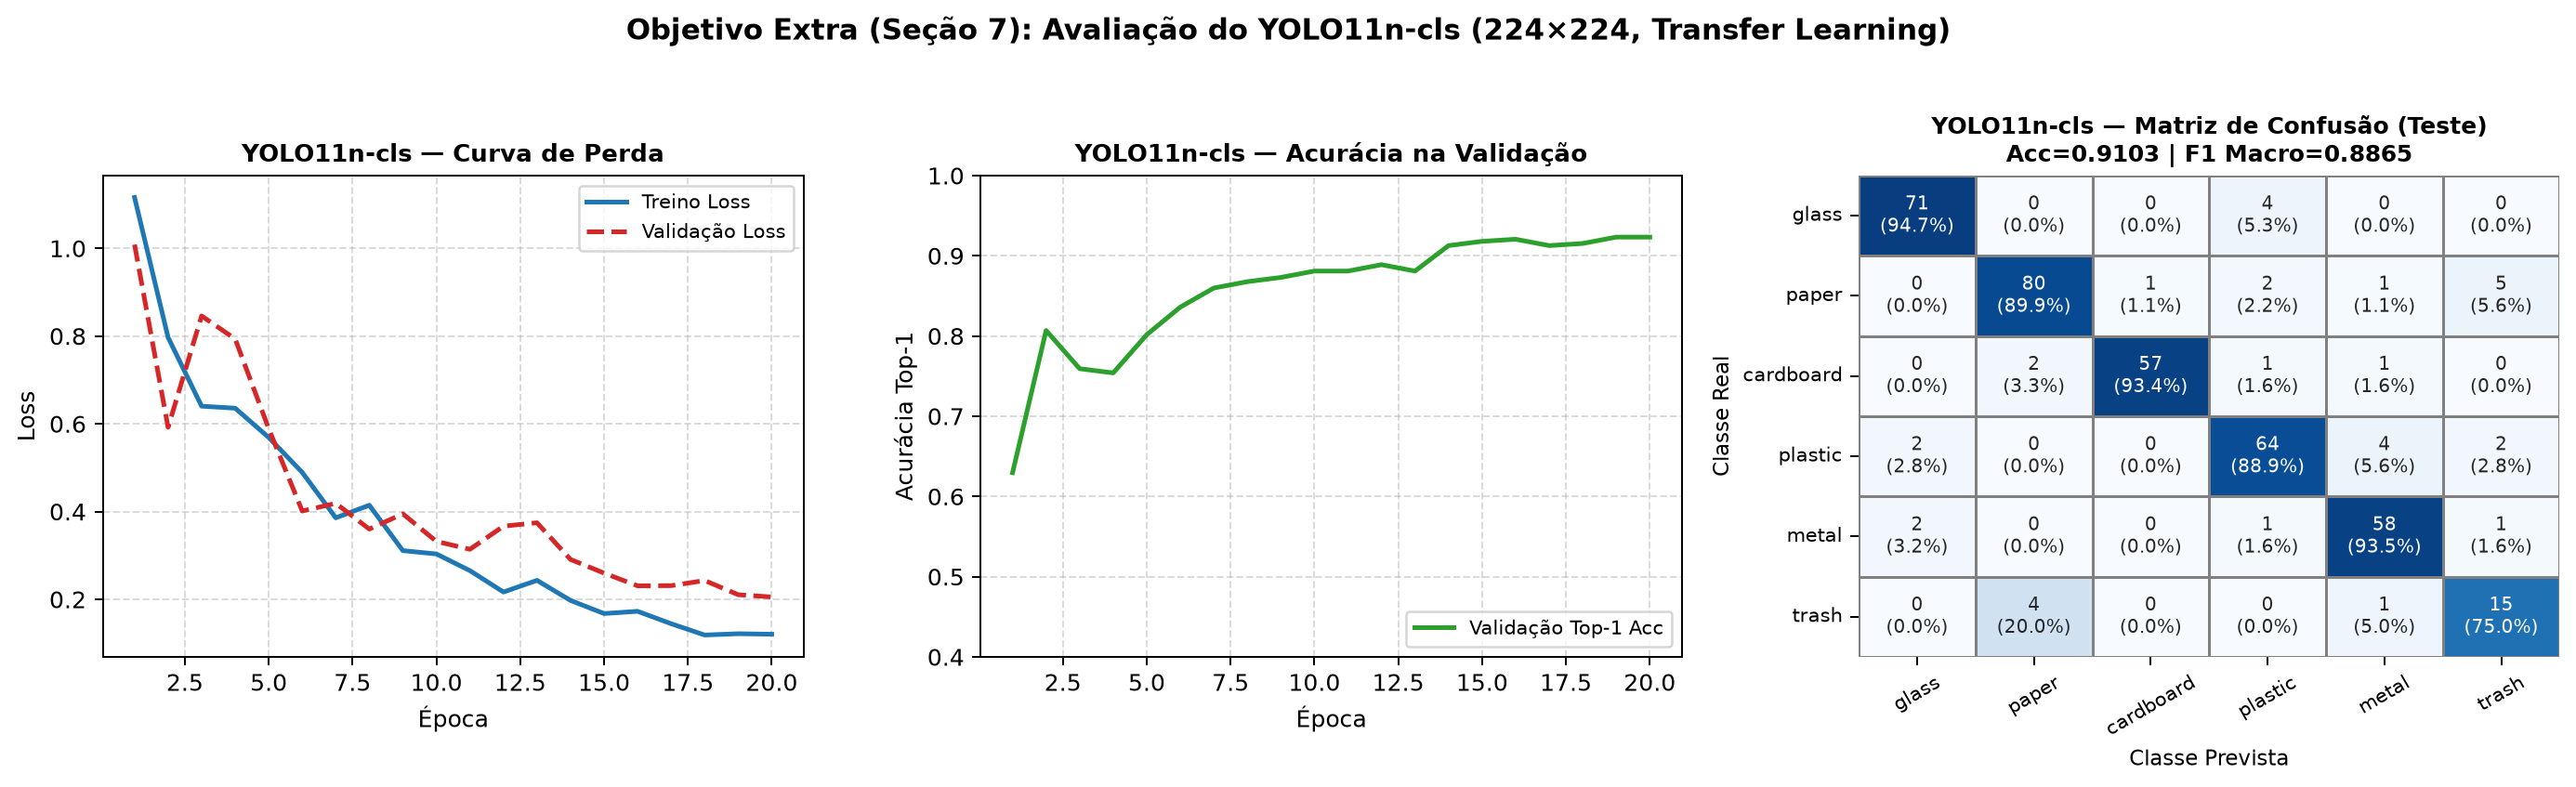
\includegraphics[width=0.98\linewidth]{fig8_yolo_bonus_avaliacao.png}\\
    {\footnotesize Fonte: Elaborada pelos autores (2026).}
\end{figure}

% ==============================================================================
\section{Discussão}
% ==============================================================================

\subsection{Arquiteturas: MLP versus CNN em $128 \times 96$}

A comparação controlada em $128 \times 96$ pixels, sob o mesmo limite de épocas, mesma paciência e mesma aumentação de dados, evidencia uma vantagem expressiva das CNNs sobre as MLPs na classificação visual. A MLP (Exp 1) possui 9.471.110 parâmetros (36,13~MB), pois conecta cada um dos 36.864 valores RGB da imagem achatada aos neurônios ocultos, perdendo a vizinhança espacial. Como consequência, a MLP estagnou logo no início (\textit{Early Stopping} na época 12, melhor época 2), obtendo 34,83\% de acurácia e 0,2275 de F1 macro no teste, com colapso completo ($\text{F1} = 0{,}00$ via \texttt{zero\_division=0}) em \textit{metal} e \textit{trash} e forte viés para \textit{paper} (\textit{recall} 0,97 com precisão 0,28). Em contraste, a CNN (Exp 3) utilizou apenas \textbf{28.358 parâmetros} (334 vezes menor e 0,12~MB em disco) graças ao compartilhamento de filtros convolucionais e ao \textit{Global Average Pooling}, alcançando 74,67\% de acurácia e 0,7154 de F1 macro no teste, reduzindo de forma consistente a perda até a época 42 (parando na 52) sem sobreajuste acentuado.

\subsection{Efeito do Desequilíbrio e dos Pesos de Classe}

A introdução de pesos inversamente proporcionais à frequência ($w_{\text{trash}} = 3{,}0625$ frente a $w_{\text{paper}} = 0{,}7067$) produziu efeitos distintos nas duas arquiteturas. Na MLP (Exp 2), o desbalanceamento ponderado instabilizou o treinamento logo na época 1 (parada na 11), levando a acurácia global para 25,86\% (F1 macro 0,1100), com \textit{recall} nulo para \textit{glass} e \textit{trash}. Na CNN (Exp 4), porém, a ponderação elevou o \textit{recall} de \textit{trash} de 0,45 para \textbf{0,60} (12 de 20 amostras corretas) e atingiu o maior F1 macro de validação entre os obrigatórios (\textbf{0,7277}), embora reduzindo a precisão de \textit{trash} (0,64 $\to$ 0,40) e gerando 73,09\% de acurácia e 0,7036 de F1 macro no teste frente a 74,67\% e 0,7154 do Exp 3, evidenciando o \textit{trade-off} entre sensibilidade e precisão em classes raras.

\subsection{Efeito da Resolução na CNN e Custo Computacional}

Graças ao \textit{Global Average Pooling}, o número de parâmetros permaneceu idêntico (28.358) nas três resoluções. Entretanto, o tempo médio por época subiu de 4,11~s ($128 \times 96$) para 21,94~s ($256 \times 192$, ${\sim}5{,}3\times$) e 93,59~s ($512 \times 384$, ${\sim}22{,}8\times$), enquanto o pico de RAM saltou de 846,0~MB para 2.112,3~MB e 6.439,6~MB. Em desempenho no teste, $256 \times 192$ obteve exatamente a mesma acurácia de $128 \times 96$ (74,67\%) com F1 macro ligeiramente maior (0,7213 contra 0,7154, diferença modesta sem teste formal de significância), mas $512 \times 384$ caiu para 70,98\% de acurácia e 0,6582 de F1 macro (melhor época 23/33), pois filtros $3\times 3$ fixos observam uma fração menor do objeto em imagens maiores. Portanto, \textbf{imagens maiores não trouxeram vantagem que justificasse o aumento de tempo e memória} nesta topologia fixa, e as medições na CPU confirmam inferência leve de 0,62~ms/imagem em $128 \times 96$ e 3,74~ms/imagem em $256 \times 192$ (18,07~ms/imagem em $512 \times 384$).

\subsection{Análise de Erros, Limitações do Dataset e Comparação com a Literatura}

Na análise de erros do Exp 4 (Figura~\ref{fig:erros}), as maiores confusões ocorreram entre \textit{glass}, \textit{plastic} e \textit{metal} (por exemplo, \texttt{glass270.jpg} previsto como \textit{plastic} com 97,9\% e \texttt{metal37.jpg} como \textit{plastic} com 93,9\%) por transparência e reflexos especulares semelhantes, e entre embalagens e rótulos impressos com fundo claro (\texttt{trash91.jpg} como \textit{paper} com 95,7\%, \texttt{cardboard33.jpg} como \textit{plastic} com 89,3\%, \texttt{paper31.jpg} como \textit{plastic} com 83,2\% e \texttt{plastic364.jpg} como \textit{paper} com 82,2%). Além da remoção prévia dos três pares duplicados conflitantes, limitações como fundo claro homogêneo e objeto único centralizado restringem o uso direto em fotografias reais sem adaptação. Comparado a Yang e Thung (2016) --- 63\% com SVM em seis classes e 22\% com CNN em cinco classes (excluindo \textit{trash}) --- e ao resultado posterior do repositório oficial (${\sim}75\%$ com CNN), nossas CNNs em $128 \times 96$ e $256 \times 192$ (74,67\% no conjunto limpo) aproximam-se da continuação do repositório, embora os valores não sejam diretamente equiparáveis devido às diferenças de classes, remoção dos 6 arquivos duplicados, divisão fixa (70/15/15), resolução e camadas de regularização.

\subsection{Discussão do Objetivo Extra: Transferência de Aprendizagem com YOLO11n-cls}

O modelo \textbf{YOLO11n-cls} (Exp 7: \textbf{91,03\% Acc}; \textbf{0,8865 F1 macro}; 0,75 de \textit{recall} em \textit{trash}; 34 erros em 379 imagens) superou em +16,36 p.p.\ as melhores CNNs obrigatórias no teste (Exp 3 e Exp 5). Esse ganho reflete os efeitos esperados de \textit{Transfer Learning} e \textit{Fine-Tuning}: a base pré-treinada no \textit{ImageNet-1K} fornece extratores visuais gerais (YOSINSKI et al., 2014), somados à arquitetura moderna C3k2 (1,54M parâmetros), resolução $224 \times 224$ e aumentação padrão do Ultralytics (JOCHER; CHAURASIA; QIU, 2024). O custo foi o tempo de ajuste fino em CPU (2.462,58~s), mantendo latência de inferência medida em 16,70~ms/imagem na mesma CPU.

% ==============================================================================
\section{Conclusão}
% ==============================================================================

Os experimentos realizados indicaram que as CNNs alcançam desempenho muito superior ao das MLPs no \textit{TrashNet} limpo (2.521 imagens) com menos de 0,3\% dos parâmetros, que os pesos de classe elevam a sensibilidade de \textit{trash} na CNN ($0{,}45 \to 0{,}60$, ao custo de menor precisão), e que o aumento de resolução para $512 \times 384$ sem aprofundamento arquitetural não melhora a acurácia no teste (70,98\% vs.\ 74,67\%) enquanto multiplica por ${\sim}22{,}8\times$ o tempo por época. O objetivo extra com \textit{YOLO11n-cls} mostrou que a transferência de aprendizagem é uma alternativa muito efetiva para bases pequenas e desbalanceadas (91,03\% de acurácia; 0,8865 F1 macro). Como trabalhos futuros, sugerem-se avaliar CNNs mais profundas em resoluções maiores, busca sistemática de hiperparâmetros com validação cruzada e validação em cenários reais com fundos complexos.

% ==============================================================================
\section*{Referências}
% ==============================================================================
\begin{flushleft}
\footnotesize
BARBOSA, Paulo Cirillo Souza. \textbf{Redes Neurais Artificiais}: Percursos de Aprendizagem 1 a 4. Fortaleza: Universidade de Fortaleza (EAD Unifor), 2025.\\[4pt]
BISHOP, Christopher M.; NASRABADI, Nasser M. \textbf{Pattern recognition and machine learning}. New York: Springer, 2006.\\[4pt]
GOODFELLOW, Ian; BENGIO, Yoshua; COURVILLE, Aaron. \textbf{Deep learning}. Cambridge: MIT Press, 2016.\\[4pt]
HAYKIN, Simon. \textbf{Redes neurais}: princípios e prática. 2. ed. Porto Alegre: Bookman, 2001.\\[4pt]
JOCHER, Glenn; CHAURASIA, Ayush; QIU, Jing. \textbf{Ultralytics YOLO11}: Classification documentation. 2024. Disponível em: \url{https://docs.ultralytics.com/tasks/classify/}. Acesso em: 22 nov. 2026.\\[4pt]
PASZKE, Adam et al. PyTorch: An imperative style, high-performance deep learning library. In: \textbf{Advances in Neural Information Processing Systems (NeurIPS)}, v. 32, 2019.\\[4pt]
RUMELHART, David E.; HINTON, Geoffrey E.; WILLIAMS, Ronald J. Learning representations by back-propagating errors. \textbf{Nature}, v. 323, p. 533-536, 1986.\\[4pt]
SILVA, Ivan Nunes da; SPATTI, Danilo Hernane; FLAUZINO, Rogério Andrade. \textbf{Redes neurais artificiais para engenharia e ciências aplicadas}. São Paulo: Artliber, 2010.\\[4pt]
YANG, Mindy; THUNG, Gary. \textbf{Classification of trash for recyclability status}. Stanford University: CS229 Project Report, 2016. Repositório e dataset disponíveis em: \url{https://github.com/garythung/trashnet}. Acesso em: 22 nov. 2026.\\[4pt]
YOSINSKI, Jason et al. How transferable are features in deep neural networks? In: \textbf{Advances in Neural Information Processing Systems (NeurIPS)}, v. 27, 2014.\\[4pt]
ZEILER, Matthew D.; FERGUS, Rob. Visualizing and understanding convolutional networks. In: \textbf{Computer Vision -- ECCV 2014}. Cham: Springer, 2014. p. 818-833.
\end{flushleft}

\end{document}
